\clearpage
\VerdierPhysicalPageAnchor{0141}%
\begingroup
\small
\setlength{\parskip}{0pt}%
\setlength{\emergencystretch}{1.5em}%
\setlength{\abovedisplayskip}{1pt plus 1pt minus 1pt}%
\setlength{\belowdisplayskip}{1pt plus 1pt minus 1pt}%

\VerdierSemanticAnchor{ch2-2-2-8-stepwise-conditions}
\noindent ただし次を満たす：

\VerdierSemanticAnchor{ch2-2-2-8-condition-1}
\par\noindent\makebox[1.8em][l]{1)}$us_1=tu_1''$ かつ $s_1\in S$。
これは SM2) を用いて得られる。

\VerdierSemanticAnchor{ch2-2-2-8-condition-2}
\par\noindent\makebox[1.8em][l]{2)}$mQ(s_1s_2)=Q(f')$。ただし
$f'\colon X_2''\longrightarrow X'$ は $\mathcal D$ の射、
$u_2''=u_1''s_2$、$s_2\in S$ である。これは定理 (2.2.2) を用いて
得られる。

\VerdierSemanticAnchor{ch2-2-2-8-condition-3}
\par\noindent\makebox[1.8em][l]{3)}$u'f's_3=gu_2''s_3$、
$u''=u_2''s_3$、$s_3\in S$。実際、$\mathcal D$ の図式

\VerdierSemanticAnchor{ch2-2-2-8-source-square}
\begin{center}
  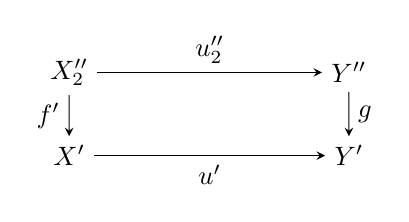
\begin{tikzpicture}[>=stealth,line width=.38pt,x=1.85cm,y=1.10cm,
    scale=.96,transform shape]
    \node (X2pp) at (0,1) {$X_2''$};
    \node (Ypp)  at (2,1) {$Y''$};
    \node (Xp)   at (0,0) {$X'$};
    \node (Yp)   at (2,0) {$Y'$};
    \draw[->] (X2pp) -- node[above] {$u_2''$} (Ypp);
    \draw[->] (X2pp) -- node[left] {$f'$} (Xp);
    \draw[->] (Ypp)  -- node[right] {$g$} (Yp);
    \draw[->] (Xp)   -- node[below] {$u'$} (Yp);
  \end{tikzpicture}
\end{center}

\VerdierSemanticAnchor{ch2-2-2-8-localized-commutativity}
\noindent は必ずしも可換ではない。しかし、この図式に関手 $Q$ を
適用して得られる $\mathcal D(S^{-1})$ の図式は可換である。したがって
$Q(u'f')=Q(gu_2'')\colon Q(X_2'')\longrightarrow Q(Y')$ である。

\VerdierSemanticAnchor{ch2-2-2-8-s3-refinement}
$\mathcal D(S^{-1})$ の射の定義により、$u'f's_3=gu_2''s_3$ を満たす射
$s_3\in S\colon X''\longrightarrow X_2''$ が存在する。

\VerdierSemanticAnchor{ch2-2-2-8-proof-complete}
補題の証明を完了するには $f=f's_3$、$s=s_1s_2s_3$ とおけばよい。

\VerdierSemanticAnchor{ch2-2-2-9}
\smallskip
\noindent\textbf{2.2.9. 定理 2.2.6 の証明の完了。}
\VerdierSemanticAnchor{ch2-2-2-9-triv-reduction}%
集合 $T$ が性質 TRIV をもつことを示せばよい。この集合は性質 TRI、
TRII、TRIII をもつことが既に分かっているので、1.2 の結果 (1.2.14)
を用いてよい。特に (1.2.4) により、与えられた射を含む $T$ の三角は
すべて同型である。したがって、命題 (1.3.2) の証明で用いたものと
同様の簡約により、性質 TRIV の証明は、$\mathcal D$ の類似の図式を
$Q$ で写して得られる $\mathcal D(S^{-1})$ の図式に帰着される。

\VerdierSemanticAnchor{ch2-2-2-9-reader-details}
この検証は容易である。詳細は読者に委ねる。

\VerdierSemanticAnchor{ch2-2-2-10}
\smallskip
\noindent\textbf{2.2.10.}\quad
$\mathcal D$ を三角圏、$\mathcal B\subseteq\mathcal D$ を充満三角部分圏、
$S(\mathcal B)$ を $\mathcal B$ に付随する乗法的系とする (2.1.15)。

\VerdierSemanticAnchor{ch2-2-2-10-quotient-category}
圏 $\mathcal D(S(\mathcal B)^{-1})$ を $\mathcal D/\mathcal B$ と書く。
圏 $\mathcal D/\mathcal B$ を\emph{$\mathcal B$ による $\mathcal D$ の
商圏}と呼ぶ。

\VerdierSemanticAnchor{ch2-2-2-10-quotient-functor}
標準関手 $Q\colon\mathcal D\longrightarrow\mathcal D/\mathcal B$ を
\emph{商関手}と呼ぶ。$F\colon\mathcal D\longrightarrow\mathcal D'$ を
三角圏（それぞれアーベル圏）への完全（それぞれコホモロジー的）関手
とする。

\VerdierSemanticAnchor{ch2-2-2-10-kernel}
$F$ により零対象へ送られる対象（それぞれ、そのすべてのシフトが
$F$ により零対象へ送られる対象）によって定まる厳密充満飽和三角部分圏を
$\operatorname{Ker}(F)$ と書き、\emph{$F$ の核}と呼ぶ
（(2.1.16)、(2.1.17)）。

\VerdierSemanticAnchor{ch2-2-2-10-p142-boundary}
\endgroup
